% Autor: Alfredo Sánchez Alberca (email:asalber@ceu.es)
% Charts that shows the purpose of Statistics
\begin{tikzpicture}[every label/.style={text=color1}]
\tikzstyle{node} = [align=center, node distance=1cm]; 
\tikzstyle{arrow} = [-latex, color2, line width=12pt];

\node (population) [label=-90:Population] at (0,0) {\includegraphics[height=2cm]{img/introduction/population.pdf}}; 
\node (sample) [label=-90:Sample] at (5,0) {
\includegraphics[height=2cm]{img/introduction/sample.png}};
\draw[arrow] (population) -- (sample) node[midway,white] {Sampling\quad\phantom{0}};
\end{tikzpicture} 